\documentclass[tikz, margin=3mm, convert=pdf2svg]{standalone}
\usetikzlibrary{calc,arrows,automata,fit,backgrounds,shadows,positioning}
\usetikzlibrary{shapes.geometric,shapes.symbols}

\begin{document}

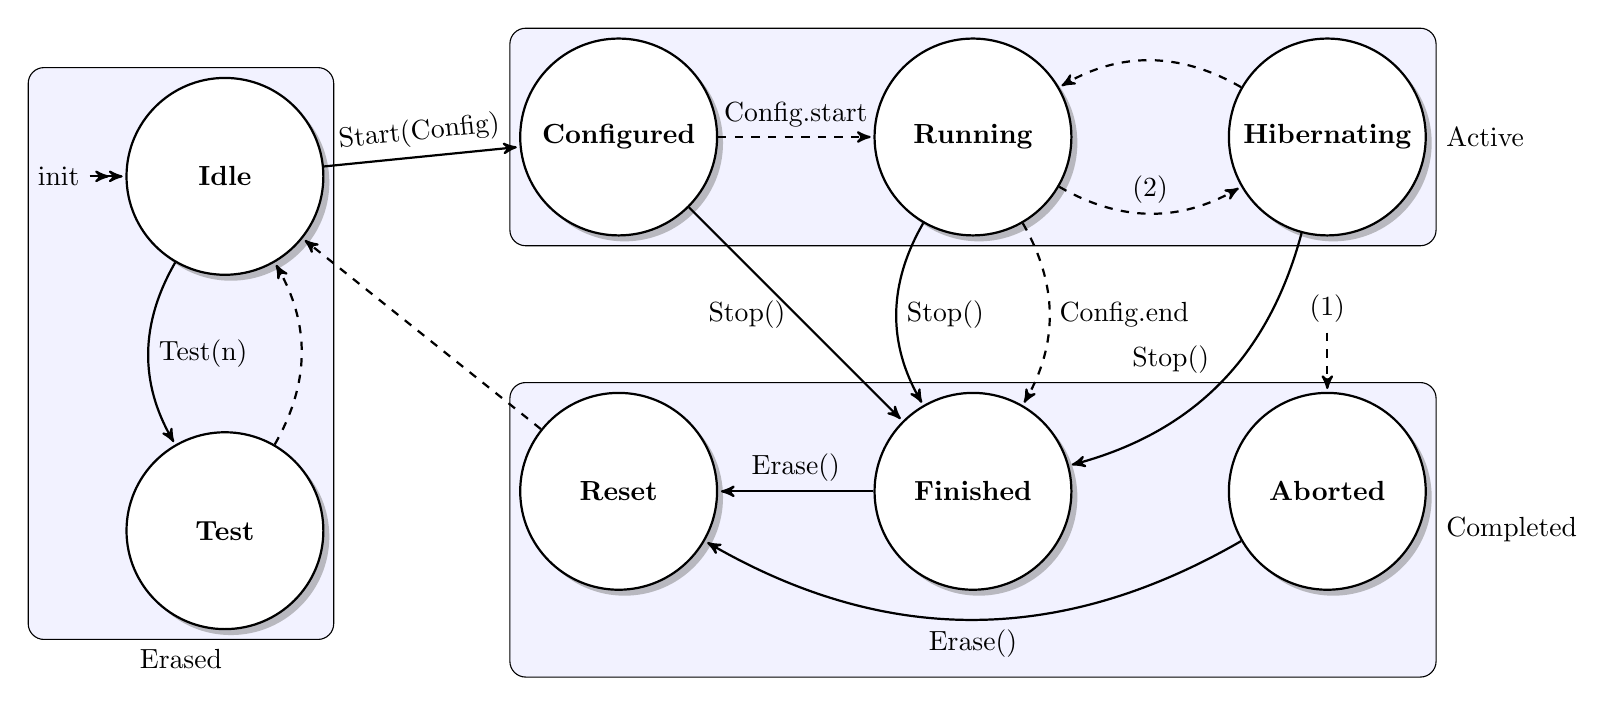
\begin{tikzpicture}[->,>=stealth',shorten >=1pt,auto,node distance=4.5cm,
  thick,state/.style={circle,draw,minimum size=2.5cm,fill=white,drop shadow},
  every initial by arrow/.style={->>},
  initial text=init]
  \tikzstyle{surround} = [fill=blue!5,draw=black,rounded corners=2mm]
%  scale=0.8, every node/.style={scale=0.8},
 
  \node (DUMMY) at (-2.25,0) {};
  \node[initial left,state]   (IDLE)    at (0,0)                   {\bf Idle};
  
   \node[state] (TEST) [below of=IDLE]  {\bf Test};
 
\node[state]           (CONFIGURED) at (5,0.5)          {\bf Configured};
  \node[state]           (RUNNING)   [right of=CONFIGURED]     {\bf Running};
\node[state]     (RESET)     [below of=CONFIGURED]           {\bf Reset};
\node[state]           (FINISHED)  [right of=RESET]     {\bf Finished};
\node[state]           (ABORTED)   [right of=FINISHED]     {\bf Aborted};

\node[state]           (HIBERNATING) [right of=RUNNING] {\bf Hibernating};
\node[] (ERROR) [above=0.75cm  of ABORTED] {(1)};
\path 
      (IDLE)      edge                 node[sloped,anchor=center,above] {Start(Config)}            (CONFIGURED)
      (CONFIGURED) edge [dashed]       node {Config.start}                                         (RUNNING)
      (CONFIGURED) edge                node [left] {Stop()}                                       (FINISHED)
      (RUNNING)   edge  [bend right]               node[right] {Stop()}                            (FINISHED)
      (RUNNING)   edge  [dashed,bend left]        node[right] {Config.end}                            (FINISHED)

      (ABORTED)   edge      [bend left]    node(l1) [below]{Erase()}                                                  (RESET)
      (FINISHED)  edge                   node [above]{Erase()}                  (RESET)
      (RESET)     edge  [dashed] (IDLE)
      (IDLE)      edge [bend right]    node {Test(n)} (TEST)
      (TEST)      edge [dashed,bend right] (IDLE)
      (RUNNING)   edge [dashed,bend right] node {(2)} (HIBERNATING)
      (HIBERNATING) edge [dashed,bend right] (RUNNING)
      (HIBERNATING) edge [bend left] node[above left] {Stop()} (FINISHED)
      (ERROR) edge [dashed] (ABORTED);

\begin{pgfonlayer}{background}
\node[surround] (background) [ fit = (CONFIGURED) (RUNNING) (HIBERNATING), label={right:Active}] {};
\node[surround] (background) [ fit = (RESET) (ABORTED) (FINISHED) (l1),label={right:Completed}] {};
\node[surround] (background) [ fit = (IDLE) (TEST) (DUMMY),label={below:Erased}] {};
\end{pgfonlayer}

\end{tikzpicture}

\end{document}

